% ========================================================================
% ========================================================================
\section*{Installation}
\href{https://auto.gluon.ai/stable/index.html}{AutoGluon} (\href{https://github.com/awslabs/autogluon/}{GitHub}) requires pip > 1.4 (upgrade by pip install -U pip). \href{https://auto.gluon.ai/stable/index.html#installation}{More installation options}. AutoGluon supports Python 3.7 to 3.9. Installation is available for Linux, MacOS, and Windows.

\begin{minted}[fontsize=\footnotesize, bgcolor=codeback, frame=leftline, framesep=10pt]{bash}
pip install autogluon
\end{minted}

% ========================================================================

\section*{Classification \& Regression}
MultiModalPredictor finetunes foundation models for solving classification and regression problems with image, text, and tabular features. Here, we use a simplified version \href{https://automl-mm-bench.s3.amazonaws.com/petfinder_for_tutorial.zip}{petfinder\_for\_tutorial} from the \href{https://www.kaggle.com/c/petfinder-adoption-prediction}{PetFinder dataset}. MultiModalPredictor automatically analyzes the columns in the input dataframe to detect categorical, numerical, text, and images (stored as paths).
\begin{minted}[fontsize=\footnotesize, bgcolor=codeback, frame=leftline, framesep=10pt]{python}
import pandas as pd
train_data = pd.read_csv(
   'petfinder_for_tutorial/train.csv', index_col=0)
test_data = pd.read_csv(
   'petfinder_for_tutorial/test.csv', index_col=0)
\end{minted}

To train the model, just call `.fit()'. We also support customization (\href{https://auto.gluon.ai/stable/tutorials/multimodal/advanced_topics/customization.html}{docs}).

\begin{minted}[fontsize=\footnotesize, bgcolor=codeback, frame=leftline, framesep=10pt]{python}
from autogluon.multimodal import MultiModalPredictor
predictor = MultiModalPredictor(
    problem_type="classification", 
    label="AdoptionSpeed"
)
predictor.fit(train_data)
predictor.fit_summary() # Summarize the model
\end{minted}

To evaluate on the validation data and run inference

\begin{minted}[fontsize=\footnotesize, bgcolor=codeback, frame=leftline, framesep=10pt]{python}
predictor.evaluate(test_data)  # Evaluation
predictor.predict(test_data)  # Inference
\end{minted}

\section*{Named-Entity Recognition}
MultiModalPredictor supports named-entity recognition. We use \href{https://groups.csail.mit.edu/sls/downloads/movie/}{MIT movies corpus} to demonstrate the usage, which can be downloaded from \href{https://automl-mm-bench.s3.amazonaws.com/ner/mit-movies/train.csv}{train.csv} and \href{https://automl-mm-bench.s3.amazonaws.com/ner/mit-movies/test.csv}{test.csv}.

\begin{minted}[fontsize=\footnotesize, bgcolor=codeback, frame=leftline, framesep=10pt]{python}
from autogluon.multimodal import MultiModalPredictor
predictor = MultiModalPredictor(
    problem_type="ner", label="entity_annotations"
)
# Train model
predictor.fit("train.csv")
# Evaluation
predictor.evaluate("test.csv")

# Inference
sentence = "Game of Thrones is an American fantasy "
           "drama television series created" 
           "by David Benioff"
predictions = predictor.predict({
    'text_snippet': [sentence]
})
\end{minted}

\section*{Object Detection}
To use MultiModalPredictor for object detection, please first install additional dependencies by
\begin{minted}[fontsize=\footnotesize, bgcolor=codeback, frame=leftline, framesep=10pt]{bash}
mim install mmcv-full
pip install mmdet
pip install pycocotools-windows # if windows users
\end{minted}

MultiModalPredictor supports common object detection data formats such as \href{http://host.robots.ox.ac.uk/pascal/VOC/}{VOC} and \href{https://cocodataset.org/}{COCO}. Here we use the dataset \href{https://automl-mm-bench.s3.amazonaws.com/object_detection_dataset/tiny_motorbike_coco.zip}{tiny$\_$motorbike\_coco} to demonstrate how to use MultiModalPredictor. The predictor natively supports json files in the COCO-format.

\begin{minted}[fontsize=\footnotesize, bgcolor=codeback, frame=leftline, framesep=10pt]{python}
train_path = "./Annotations/trainval_cocoformat.json"
test_path = "./Annotations/test_cocoformat.json"

from autogluon.multimodal import MultiModalPredictor
model = "faster_rcnn_r50_fpn_2x_coco"
predictor = MultiModalPredictor(
    problem_type="object_detection",
    # Set the backbone. This is optional.
    hyperparameters={
        "model.mmdet_image.checkpoint_name": model,
    },
    sample_data_path=train_path,
)
\end{minted}

To train an object detector,
\begin{minted}[fontsize=\footnotesize, bgcolor=codeback, frame=leftline, framesep=10pt]{python}
predictor.fit(train_path)
\end{minted}

More options for the \textbf{fit} method (\href{https://auto.gluon.ai/stable/api/autogluon.predictor.html#autogluon.multimodal.MultiModalPredictor.fit}{docs}):

\begin{minted}[fontsize=\footnotesize, bgcolor=codeback, frame=leftline, framesep=10pt]{python}
predictor.fit(train_path,
    # Limit the training time, in second
    time_limit=600,
    # Use a separate dataset to tune models.
    tuning_data=val_data
)
\end{minted}

Once trained, we can evaluate it on the test set to obtain metrics, 
\begin{minted}[fontsize=\footnotesize, bgcolor=codeback, frame=leftline, framesep=10pt]{python}
predictor.evaluate(test_path)
\end{minted}

We can also predict on any image and visualize the detected bounding boxes with its confidence scores, 
\begin{minted}[fontsize=\footnotesize, bgcolor=codeback, frame=leftline, framesep=10pt]{python}
pred = predictor.predict({"image": [test_image]})
\end{minted}

\begin{center}
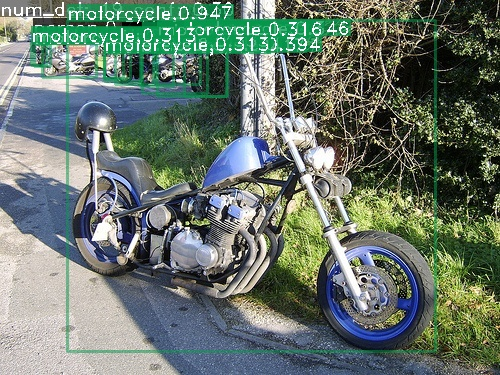
\includegraphics[width=0.6\linewidth]{images/tiny_motorbike.png}
\end{center}

\section*{Matching}
MultiModalPredictor implements a flexible twin-tower architecture that can solve text-text, image-image, and text-image matching problems (\href{https://auto.gluon.ai/stable/tutorials/multimodal/matching/index.html}{docs}). Example of extracting embeddings for semantic text matching:
\begin{minted}[fontsize=\footnotesize, bgcolor=codeback, frame=leftline, framesep=10pt]{python}
!pip install ir_datasets # Install dataset package
from autogluon.multimodal import MultiModalPredictor
from autogluon.multimodal import utils
import ir_datasets
import pandas as pd
dataset = ir_datasets.load("beir/fiqa/dev")
docs_df = pd.DataFrame(dataset.docs_iter()) \
            .set_index("doc_id")
model = "sentence-transformers/all-MiniLM-L6-v2"
predictor = MultiModalPredictor(
    problem_type="text_similarity",
    hyperparameters={
        "model.hf_text.checkpoint_name": model,
    }
)
doc_embedding = predictor.extract_embedding(docs_df)
q_embedding = predictor.extract_embedding([
    "what happened when the dot com bubble burst?"
])
similarity = utils.compute_semantic_similarity(
    q_embedding, doc_embedding
)
# Get the most relevant document
docs_df['text'].iloc[similarity.argmax().numpy()]
\end{minted}

In addition, you can finetune the matching model via relevance data. Here, we demonstrate the use-case via the \href{https://paperswithcode.com/dataset/flickr30k}{Flickr30K} image-text matching dataset preprocessed in the dataframe format: \href{https://automl-mm-bench.s3.amazonaws.com/flickr30k.zip}{flickr30k.zip}.
\begin{minted}[fontsize=\footnotesize, bgcolor=codeback, frame=leftline, framesep=10pt]{python}
import pandas as pd
train_data = pd.read_csv("train.csv", index_col=0)
tdata = pd.read_csv("test.csv", index_col=0)
\end{minted}

To finetune model, just specify the ``query" and ``response'' keys when creating predictor and pick ``image\_text\_similarity'' as problem type.
\begin{minted}[fontsize=\footnotesize, bgcolor=codeback, frame=leftline, framesep=10pt]{python}
from autogluon.multimodal import MultiModalPredictor
predictor = MultiModalPredictor(
            query="caption",
            response="image",
            problem_type="image_text_similarity",
        )
predictor.fit(train_data, time_limit=180)
e_i = predictor.extract_embedding(tdata["image"])
e_t = predictor.extract_embedding(tdata["caption"])
\end{minted}

\begin{itemize}
  \item MultiModalPredictor also supports knowledge distillation (\href{https://auto.gluon.ai/stable/tutorials/multimodal/advanced_topics/model_distillation.html}{docs}), parameter-efficient finetune (\href{https://auto.gluon.ai/stable/tutorials/multimodal/advanced_topics/efficient_finetuning_basic.html}{docs}), and HPO (\href{https://auto.gluon.ai/stable/tutorials/multimodal/advanced_topics/hyperparameter_optimization.html}{docs}).
  \item For deployment, check \href{https://auto.gluon.ai/stable/tutorials/cloud_fit_deploy/index.html}{AutoGluon-Cloud}.
  \item For other use-cases, check
  \href{https://auto.gluon.ai/stable/tutorials/tabular_prediction/index.html}{TabularPredictor} and
  \href{https://auto.gluon.ai/stable/tutorials/timeseries/index.html}{TimeSeriesPredictor}.
  \item Check the \href{https://auto.gluon.ai/stable/cheatsheet.html}{latest version of this cheat sheet}.
  \item Any questions? \href{https://github.com/awslabs/autogluon/discussions}{Ask here}
  \item Like what you see? Consider \href{https://github.com/awslabs/autogluon/stargazers}{starring AutoGluon on GitHub} and \href{https://twitter.com/autogluon}{following us on twitter} to get notified of the latest updates!
\end{itemize}

% ========================================================================

\raggedcolumns


% \begin{minted}[fontsize=\footnotesize, bgcolor=codeback, frame=leftline, framesep=10pt]{python}
% \end{minted}
